\chapter{Unit Tests}

Bei der Erstellung der Tests wurde stets versucht die ATRIP-Regeln zu beachten. Die einzelnen Punkte sind im folgenden genauer aufgeführt.

\paragraph{Automatic}
Damit die Tests eigenständig ablaufen und ihre Ergebnisse selbst überprüfen, wird xUnit verwendet. D.h. die Tests werden als \glqq Fact\grqq{} annotiert und können dann automatisch ausgeführt werden. Es sind keine Benutzereingaben bei den Tests erforderlich und sie liefern immer das Ergebnis \glqq bestanden\grqq{} oder \glqq nicht bestanden\grqq{}.

\begin{figure}[htb]
\centering
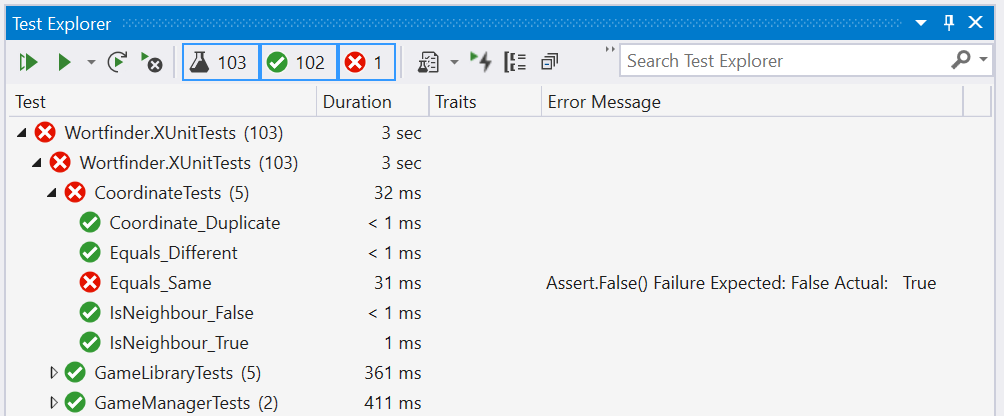
\includegraphics[width=.7\textwidth]{Bilder/TestExplorer.PNG}
\caption{\label{Abb:TestExplorer}Der Testexplorer mit bestandenen und nicht bestandenen Tests}
\end{figure}

\paragraph{Thorough}
Der Fokus wurde darauf gelegt das Wichtigste zu testen. Allerdings sind auch manche weniger relevanten Klassen abgedeckt, welche sich einfach Testen lassen und die Test Erstellung daher schnell ging. Ein Beispiel dafür ist der \href{https://github.com/EinToni/Wortfinder/blob/main/Wortfinder/GameScore.cs}{\textit{GameScore}}, welcher die Punkte des aktuellen Spiels zählt, somit nicht Missions-kritisch ist, aber dennoch abgedeckt wurde. Es wurde allerdings auch nicht jede wichtige Funktionalität getestet. Beispiele hierfür sind die GUI Elemente, welche nicht mit Tests abgedeckt sind.
%% Mehrere Szenarien abgedeckt

\paragraph{Repeatable}
Durch die Nutzung von xUnit lassen sich die Tests jederzeit auf Knopfdruck automatisch ausführen. Die Tests haben, insofern keine Änderungen im Code durchgeführt wurden, bis zum aktuellen Zeitpunkt immer das gleiche Ergebnis geliefert und sollten dies auch weiterhin, da keine direkten Festplattenzugriffe oder zeitabhängige Funktionen getestet wurden.

\paragraph{Independent}
Die Tests sind unabhängig voneinander und weisen keine impliziten Abhängigkeiten zwischen einander auf. Außerdem werden sie durch xUnit in einer unbekannten und nicht vorhersagbaren Reihenfolge ausgeführt.

\paragraph{Professional}
Es wurde versucht den Testcode möglichst einfach, leserlich und kurz zu halten. Für das bessere Verständnis wurden meistens erklärende Variablen eingeführt, anstelle die Werte direkt zu verwenden. Allerdings wurde im Nachhinein festgestellt, dass dies nicht immer eingehalten wurde. Vor allem bei sehr kurzen Tests wurde auf extra Variablen verzichtet. In der folgenden Abbildung sieht man links einen einfach verständlichen Test mit extra Variablen und rechts einen Test ohne extra Variablen, welcher aber aufgrund der kürze immer noch sehr verständlich ist.

\begin{figure}[!htb]
\centering
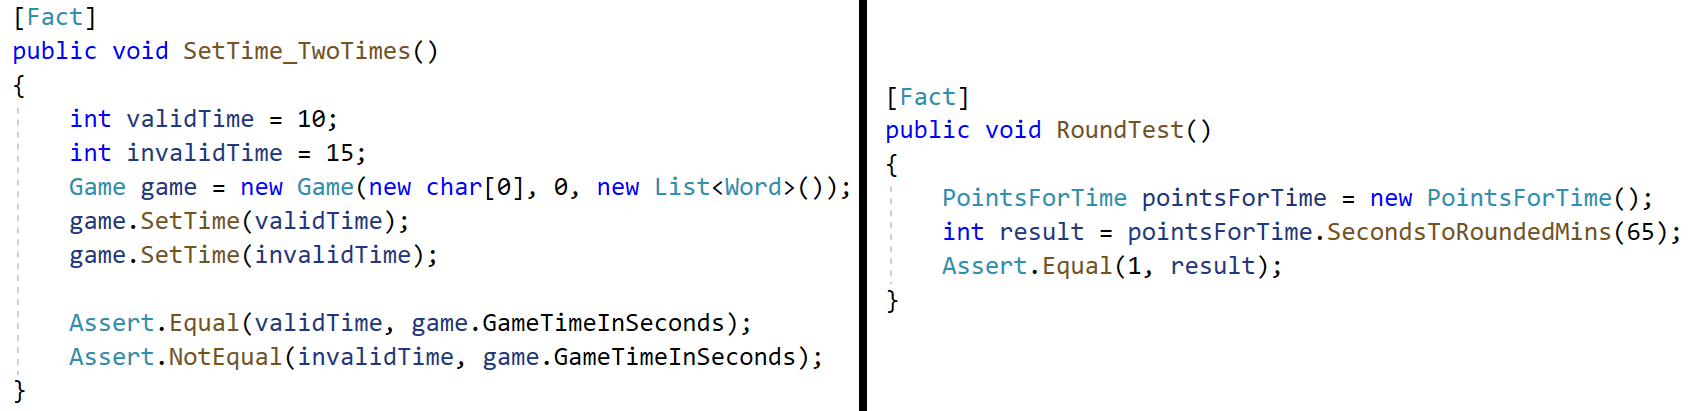
\includegraphics[width=0.95\textwidth]{Bilder/professional_example.PNG}
\caption{\label{Abb:professional_example} Professional Beispiel in ATRIP}
\end{figure}


\paragraph{Struktur}
Die Tests wurden in der AAA-Normalform erstellt. Ein Beispiel für die Normalform ist in der folgenden Abbildung dargestellt. Dabei werden im \glqq Arrange\grqq{} Part zwei Variablen instantiiert und anschließend zwei Objekte der zu testenden Klasse erstellt. Danach folgt der \glqq Act\grqq{} Part, d.h. die Ausführung, in dem die zu testende Funktion der Klasse aufgerufen und der Rückgabewert gespeichert wird. Abschließend folgt noch der \glqq Assert\grqq{} Teil, in welchem Überprüft wird, ob das erwartete Ergebnis vorliegt.


In dem dargestellten Test wird die Funktion zur Bestimmung der Nachbarschaft zweier Koordinaten geprüft. Dabei werden zwei Koordinaten erstellt welche keine Nachbarn sind und die Funktion \glqq IsNeighbour\grqq{} des einen Objekts mit dem anderen Objekt als Parameter aufgerufen. Da sie keine Nachbarn sind wird auch beim Assert ein False erwartet.

\begin{figure}[!htb]
\centering
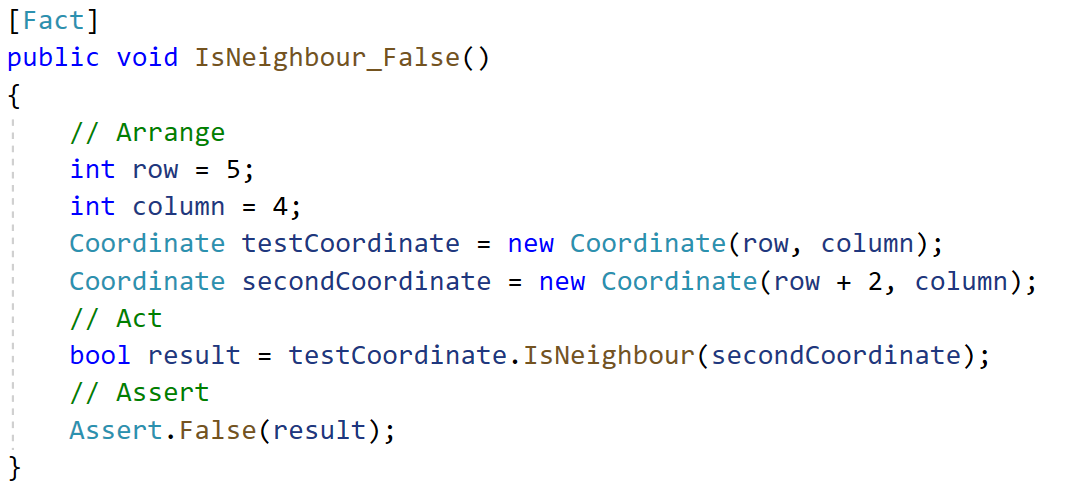
\includegraphics[width=0.65\textwidth]{Bilder/UnitTest2.PNG}
\caption{\label{Abb:UnitTest}Beispiel Test in AAA-Normalform}
\end{figure}

Ein Beispiel für einen Test mit Mock-Objekten ist nachfolgend dargestellt. Für die Erstellung von Mocks wurde Moq verwendet. Bei der Normalform für Mocks kommt noch ein \glqq Capture\grqq{}  und \glqq Verify\grqq{} Part dazu. Im Capture Teil werden die Mocks erstellt und Konfiguriert, d.h. es wird bestimmt was bei welchen Funktionsaufrufen zurückgegeben werden soll. Im Verify Teil wird überprüft, ob die konfigurierten Funktionen der Mocks auch wirklich aufgerufen wurden. Dazwischen sind die bereits beschriebenen Arrange-, Act- und Assert-Parts.

In dem dargestellten Test wird geprüft ob der \href{https://github.com/EinToni/Wortfinder/blob/main/Wortfinder/ScoreManager.cs}{\textit{ScoreManager}} bei einem Aufruf der \glqq GetTopScores\grqq{}-Funktion den \href{https://github.com/EinToni/Wortfinder/blob/main/Wortfinder/ScoreDataController.cs}{\textit{ScoreDataController}} aufruft und bei einer leeren Liste ebenfalls eine leere Liste zurück gibt.

\begin{figure}[!htb]
\centering
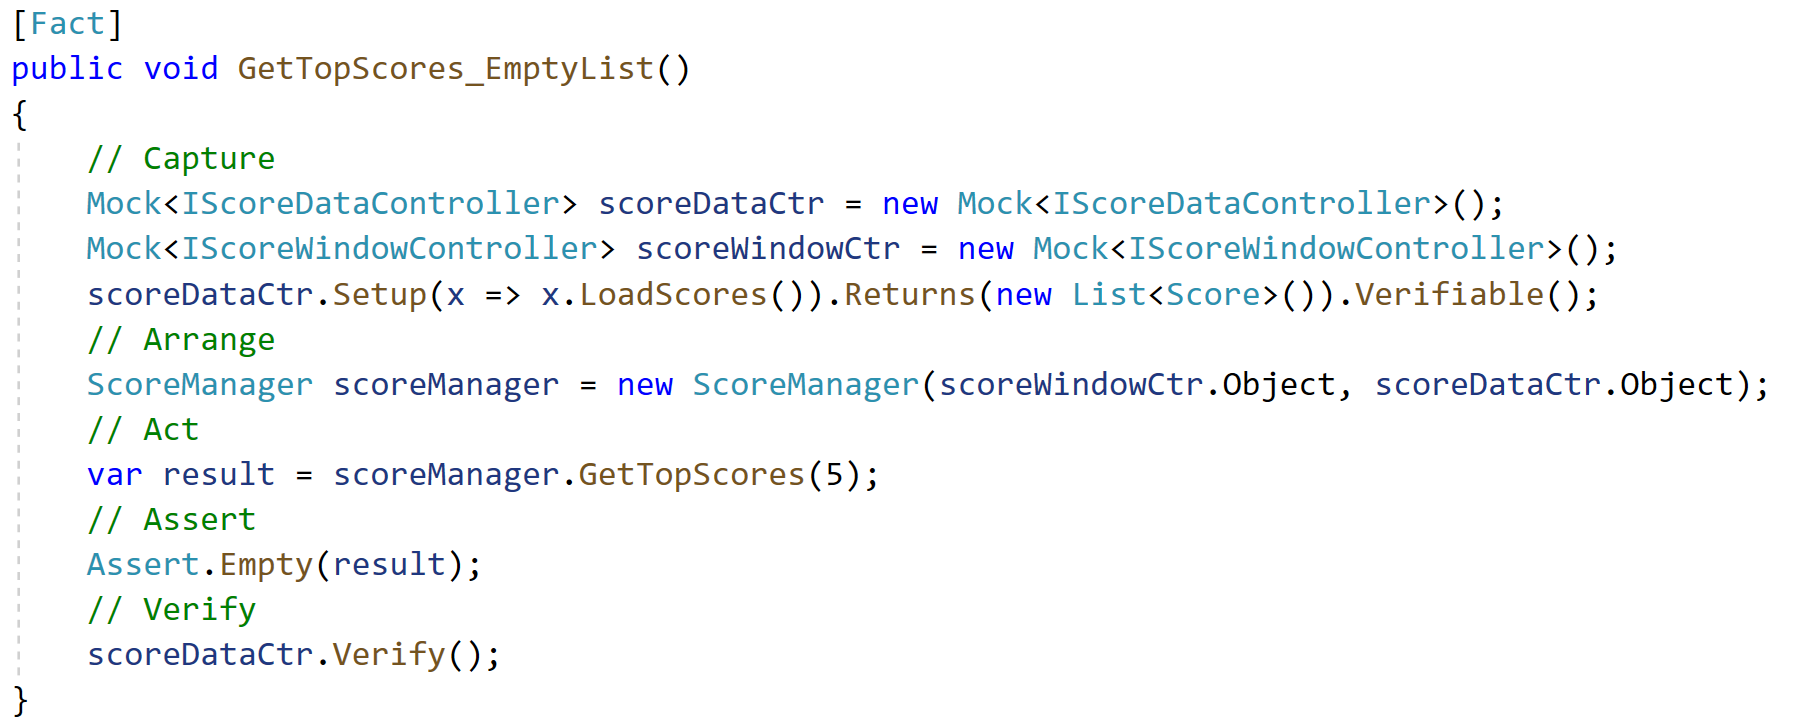
\includegraphics[width=0.8\textwidth]{Bilder/UnitTestVerify.PNG}
\caption{\label{Abb:UnitTestMocks}Beispiel Test mit Mocks}
\end{figure}

\paragraph{Code-Coverage} Zur Bestimmung der Test Abdeckung wurde die diesbezügliche Funktionalität in Visual Studio Enterprise verwendet, welche aufgrund der Studenten Lizenz zur Verfügung steht. Die Testabdeckung der Anwendung beträgt ca. 50\% Line Coverage. Im nachfolgenden Ergebnisausschnitt dürfen dabei nur die Prozentangaben in der blau markierte Zeile beachtet werden, da dies das Projekt mit dem Anwendungscode ist.

\begin{figure}[!htb]
\centering
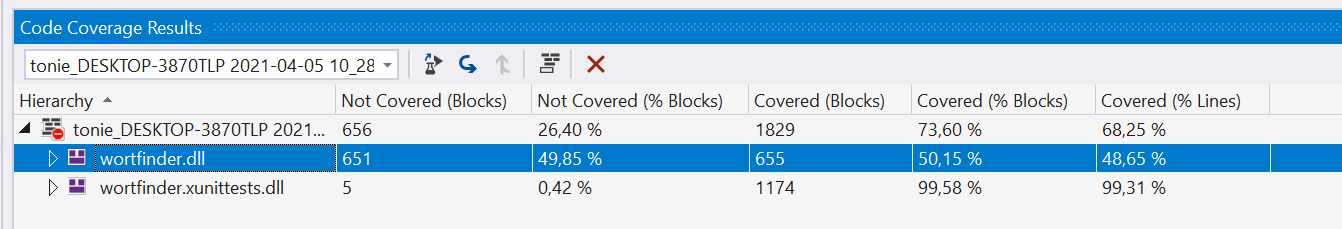
\includegraphics[width=0.95\textwidth]{Bilder/Testabdeckung.PNG}
\caption{\label{Abb:Testabdeckung}Die Ausgabe der Testabdeckung von Visual Studio}
\end{figure}

Die Abdeckung ist nicht höher, da ein großer Anteil der Codezeilen in den \textit{xaml} Dateien der GUI sind, welche nicht abgedeckt und nicht Unit-Testbar sind. Außerdem sind, wie bereits erwähnt, primär die wichtigen Stellen im Quellcode mit Tests abgedeckt. Unwichtigere werden eher vernachlässigt. Die Abdeckung könnte somit noch erhöht werden, wäre aber mit viel Aufwand verbunden welcher hier als nicht vertretbar angesehen wird.

\endinput